\documentclass[10pt]{article}
\usepackage[T1]{fontenc}
\usepackage{lmodern,amsmath,amssymb,booktabs,array,graphicx,tikz,pgfplots}
\usepackage[paperwidth=190mm,paperheight=224mm,margin=10mm]{geometry}
\usepackage[hidelinks]{hyperref}
\hypersetup{pdfauthor={},pdftitle={Monochrome mathematical illustrations: semiconductor-health identifiability}}
\usetikzlibrary{arrows.meta,positioning,calc,patterns}
\pgfplotsset{compat=1.18}
\newcommand{\trans}{^{\mathsf T}}\newcommand{\R}{\mathbb R}
\newcommand{\one}{\mathbf 1}\newcommand{\zero}{\mathbf 0}
\DeclareMathOperator{\rank}{rank}\DeclareMathOperator{\range}{range}
\DeclareMathOperator{\diag}{diag}\DeclareMathOperator{\Cov}{Cov}
\DeclareMathOperator{\Var}{Var}\DeclareMathOperator{\spanop}{span}
\newcommand{\FigureNote}{Visualization code prepared with assistance from OpenAI Codex.}
\pagestyle{empty}\setlength{\parindent}{0pt}
\tikzset{
 every picture/.style={font=\fontsize{9}{11}\selectfont,>=Latex},
 every node/.style={font=\fontsize{9}{11}\selectfont,inner sep=2pt},
 head/.style={font=\fontsize{9.5}{12}\selectfont\bfseries,anchor=west},
 tinytext/.style={font=\fontsize{8}{10}\selectfont},eq/.style={align=center},
 wire/.style={draw=black,line width=.5pt},arr/.style={->,black,line width=.65pt},
 device/.style={draw,fill=white,minimum width=1.1cm,minimum height=.38cm}}
\pgfplotsset{mathaxis/.style={axis lines=left,axis line style={black,line width=.5pt},
 tick style={black},tick label style={font=\fontsize{8}{10}\selectfont},
 label style={font=\fontsize{8.5}{10}\selectfont},grid=major,
 major grid style={black!15,line width=.2pt},
 legend style={font=\fontsize{8}{10}\selectfont,draw=none,fill=white},
 every axis plot/.append style={black}}}
\newcommand{\PlateTitle}[2]{\small\textbf{Mathematical plate #1}\hfill Monochrome TikZ / PGFPlots\par
 \vspace{1.5mm}{\large\bfseries #2}\par\vspace{2mm}}
\newcommand{\PlateCaption}[1]{\par\vspace{1mm}{\fontsize{8.5}{10.5}\selectfont #1\par
 \vspace{1mm}\FigureNote\par}}

\begin{document}
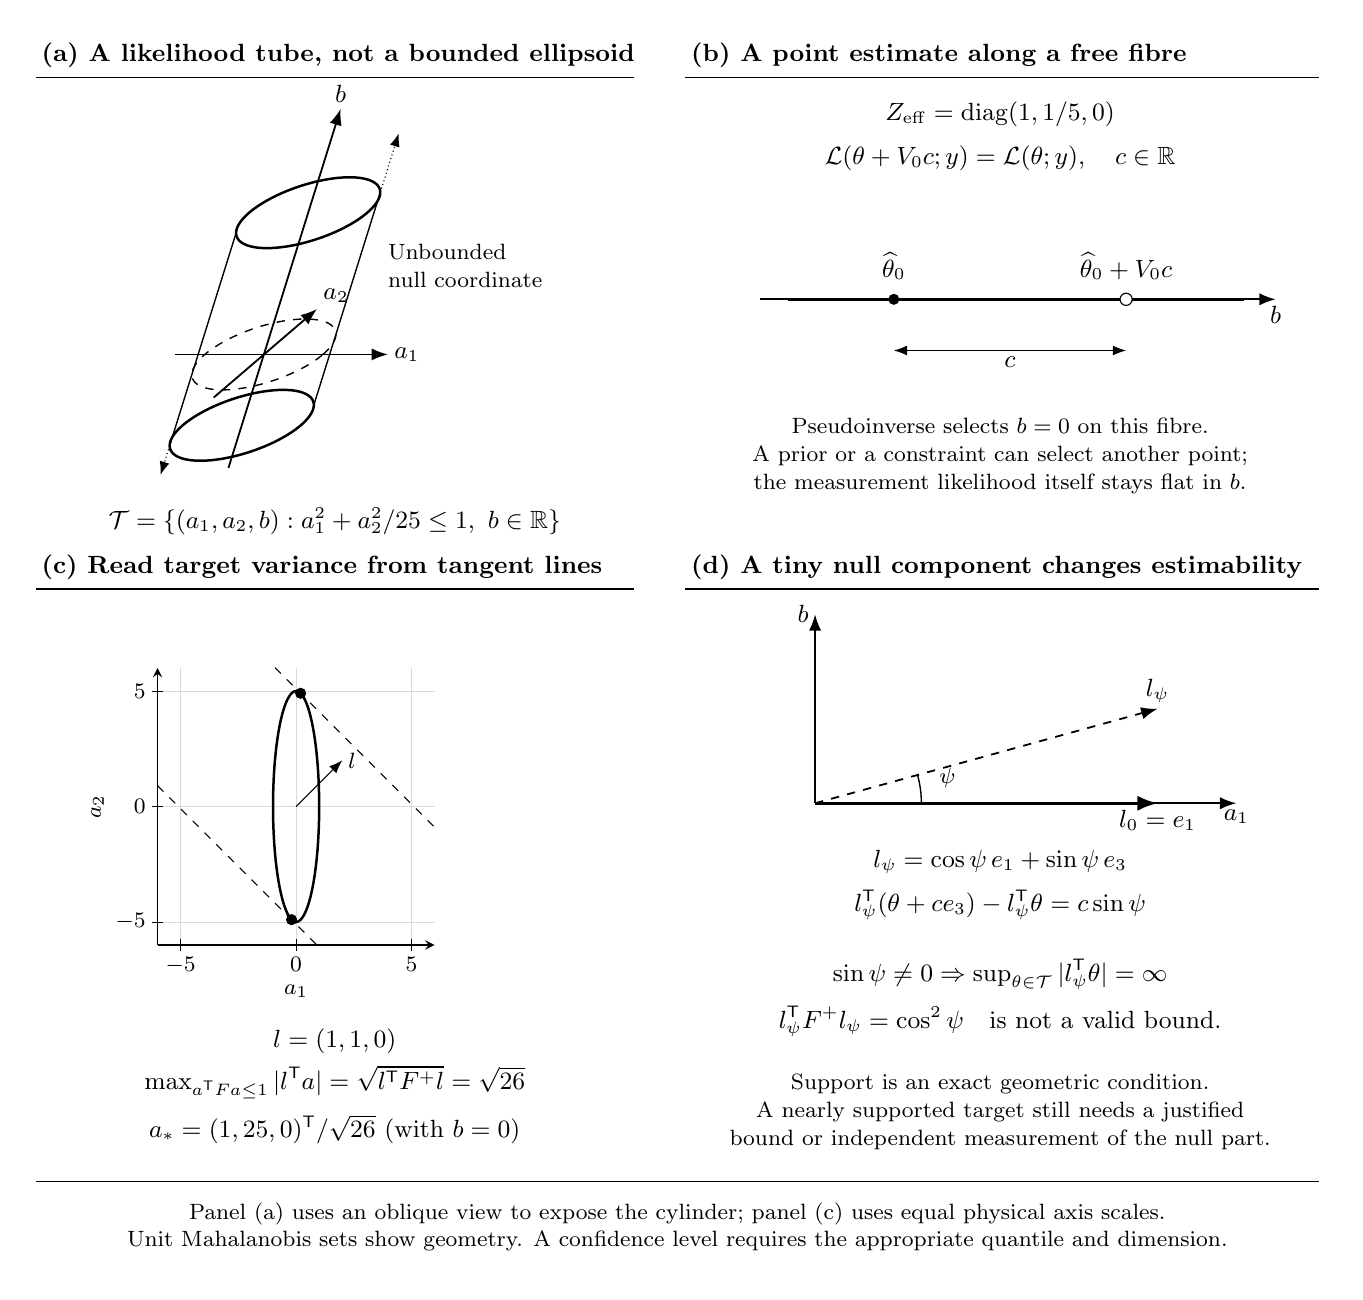
\begin{tikzpicture}[x=1cm,y=1cm]\path[use as bounding box] (0,0) rectangle (16.6,15.8);
\node[head] at (0.1,15.45){(a) A likelihood tube, not a bounded ellipsoid};\draw[wire] (0.1,15.17)--(7.699999999999999,15.17);
\node[head] at (8.35,15.45){(b) A point estimate along a free fibre};\draw[wire] (8.35,15.17)--(16.4,15.17);
\begin{scope}[shift={(3.0,11.65)},scale=.75]
\draw[arr] (-1.5,0)--(2.1,0) node[right] {$a_1$};
\draw[arr] (-.85,-.73)--(.9,.77) node[above right] {$a_2$};
\draw[arr] (-.6,-1.92)--(1.3,4.16) node[above] {$b$};
\draw[dashed,wire] plot[domain=0:360,samples=100] ({cos(\x)+.7*sin(\x)},{.6*sin(\x)});
\draw[line width=.9pt] plot[domain=0:360,samples=100] ({.75+cos(\x)+.7*sin(\x)},{2.4+.6*sin(\x)});
\draw[line width=.9pt] plot[domain=0:360,samples=100] ({-.375+cos(\x)+.7*sin(\x)},{-1.2+.6*sin(\x)});
\draw[wire] (-1.596,-1.544)--(-.471,2.056);
\draw[wire] (.846,-.856)--(1.971,2.744);
\draw[densely dotted,->] (1.971,2.744)--(2.284,3.744);
\draw[densely dotted,->] (-1.596,-1.544)--(-1.75,-2.04);
\node[tinytext,align=left,anchor=west] at (2.0,1.5){Unbounded\\null coordinate};
\end{scope}
\node[eq] at (3.9,9.53){$\mathcal T=\{(a_1,a_2,b):a_1^2+a_2^2/25\leq1,\ b\in\R\}$};
\draw[arr] (9.3,12.35)--(15.85,12.35) node[below] {$b$};
\draw[line width=.95pt] (9.65,12.35)--(15.45,12.35);
\fill (11.0,12.35) circle(2pt);\draw[fill=white] (13.95,12.35) circle(2.2pt);
\node[above] at (11,12.52){$\widehat\theta_0$};\node[above] at (13.95,12.52){$\widehat\theta_0+V_0c$};
\draw[<->] (11,11.7)--(13.95,11.7) node[midway,below] {$c$};
\node[eq] at (12.35,14.42){$Z_{\mathrm{eff}}=\diag(1,1/5,0)$\\[5pt]
$\mathcal L(\theta+V_0c;y)=\mathcal L(\theta;y),\quad c\in\R$};
\node[tinytext,align=center] at (12.35,10.36){Pseudoinverse selects $b=0$ on this fibre.\\A prior or a constraint can select another point;\\the measurement likelihood itself stays flat in $b$.};
\node[head] at (0.1,8.95){(c) Read target variance from tangent lines};\draw[wire] (0.1,8.67)--(7.699999999999999,8.67);
\node[head] at (8.35,8.95){(d) A tiny null component changes estimability};\draw[wire] (8.35,8.67)--(16.4,8.67);
\begin{axis}[mathaxis,axis equal image,at={(1.65cm,4.15cm)},anchor=south west,width=6.5cm,height=5.1cm,
 xmin=-6,xmax=6,ymin=-6,ymax=6,xtick={-5,0,5},ytick={-5,0,5},xlabel={$a_1$},ylabel={$a_2$}]
\addplot[domain=0:360,samples=120,line width=.9pt] ({cos(x)},{5*sin(x)});
\addplot[domain=-6:6,samples=2,dashed]{sqrt(26)-x};
\addplot[domain=-6:6,samples=2,dashed]{-sqrt(26)-x};
\addplot[only marks,mark=*,mark size=1.8pt] coordinates {(.196116,4.902903)(-.196116,-4.902903)};
\draw[->] (axis cs:0,0)--(axis cs:2,2);
\node[tinytext,anchor=west] at (axis cs:2,2){$l$};\end{axis}
\node[eq] at (3.9,2.35){$l=(1,1,0)$\\[4pt]
$\max_{a\trans Fa\leq1}|l\trans a|=\sqrt{l\trans F^+l}=\sqrt{26}$\\[5pt]
$a_*=(1,25,0)\trans/\sqrt{26}$ (with $b=0$)};
\draw[arr] (10,5.95)--(15.35,5.95) node[below] {$a_1$};
\draw[arr] (10,5.95)--(10,8.35) node[left] {$b$};
\draw[arr,line width=.95pt] (10,5.95)--(14.35,5.95) node[below] {$l_0=e_1$};
\draw[arr,dashed] (10,5.95)--(14.35,7.15) node[above] {$l_\psi$};
\draw[wire] (11.35,5.95) arc[start angle=0,end angle=15.4,radius=1.35];
\node[tinytext] at (11.68,6.27){$\psi$};
\node[eq] at (12.35,4.91){$l_\psi=\cos\psi\,e_1+\sin\psi\,e_3$\\[5pt]
$l_\psi\trans(\theta+ce_3)-l_\psi\trans\theta=c\sin\psi$};
\node[eq] at (12.35,3.48){$\sin\psi\neq0\Rightarrow\sup_{\theta\in\mathcal T}|l_\psi\trans\theta|=\infty$\\[5pt]
$l_\psi\trans F^+l_\psi=\cos^2\psi\quad\text{is not a valid bound.}$};
\node[tinytext,align=center] at (12.35,2.03){Support is an exact geometric condition.\\A nearly supported target still needs a justified\\bound or independent measurement of the null part.};
\draw[wire] (.1,1.15)--(16.4,1.15);
\node[tinytext,align=center] at (8.25,.57){Panel (a) uses an oblique view to expose the cylinder; panel (c) uses equal physical axis scales.\\Unit Mahalanobis sets show geometry. A confidence level requires the appropriate quantile and dimension.};
\end{tikzpicture}
\end{document}
